\documentclass{beamer}
\usetheme{Boadilla}

\title{Digital Forensics}
\subtitle{File System Forensics Masterclass}
\author{Fraser Brown}
\institute{Heriot-Watt University}
\date{\today}

\graphicspath{{../figures/}}

\begin{document}

\begin{frame}
\titlepage
\end{frame}

\begin{frame}
\section*{Overview}
\frametitle{Outline}
\tableofcontents
\end{frame}

\begin{frame}
	\frametitle{What is Digital Forensics}
	\section{What is Digital Forensics?}
%	\begin{itemize}
%		\item Digital forensics is a pulls from both cyber security and forensic science fields.
%	\end{itemize}
	\begin{block}{Digital Forensics:}
		``Computer [Digital] Forensics is the practice of determining the past actions that have taken place on a computer system using forensic techniques and understanding artefacts.'' - David Cowen
	\end{block}
		
	\begin{block}{Artefact:}
		``An Artefact is a reproducible file, setting or system change that occurs every time an application or operating system performs a specific action'' - David Cowen
	\end{block}

	The artefacts we will be dealing with in the lab are files and file systems.
\end{frame}

\begin{frame}[allowframebreaks]
	\frametitle{Why File System Analysis?}
	\subsection*{Why File System Analysis?}
	\begin{itemize}
		\item There are many different forms of digital forensic analysis:
			\begin{itemize}
				\item Network Analysis,
				\item Live memory (RAM) Analysis, 
				\item File system analysis, 
				\item Database Analysis,
				\item Application/OS Analysis
			\end{itemize}
			\item File system analysis allows:
			\begin{itemize}
				\item Introduction to a new field using a common ground
				\item Insight into how OS files relate to memory and what creation and deletion features actual do
			\end{itemize}
	\end{itemize}
	\begin{figure}
		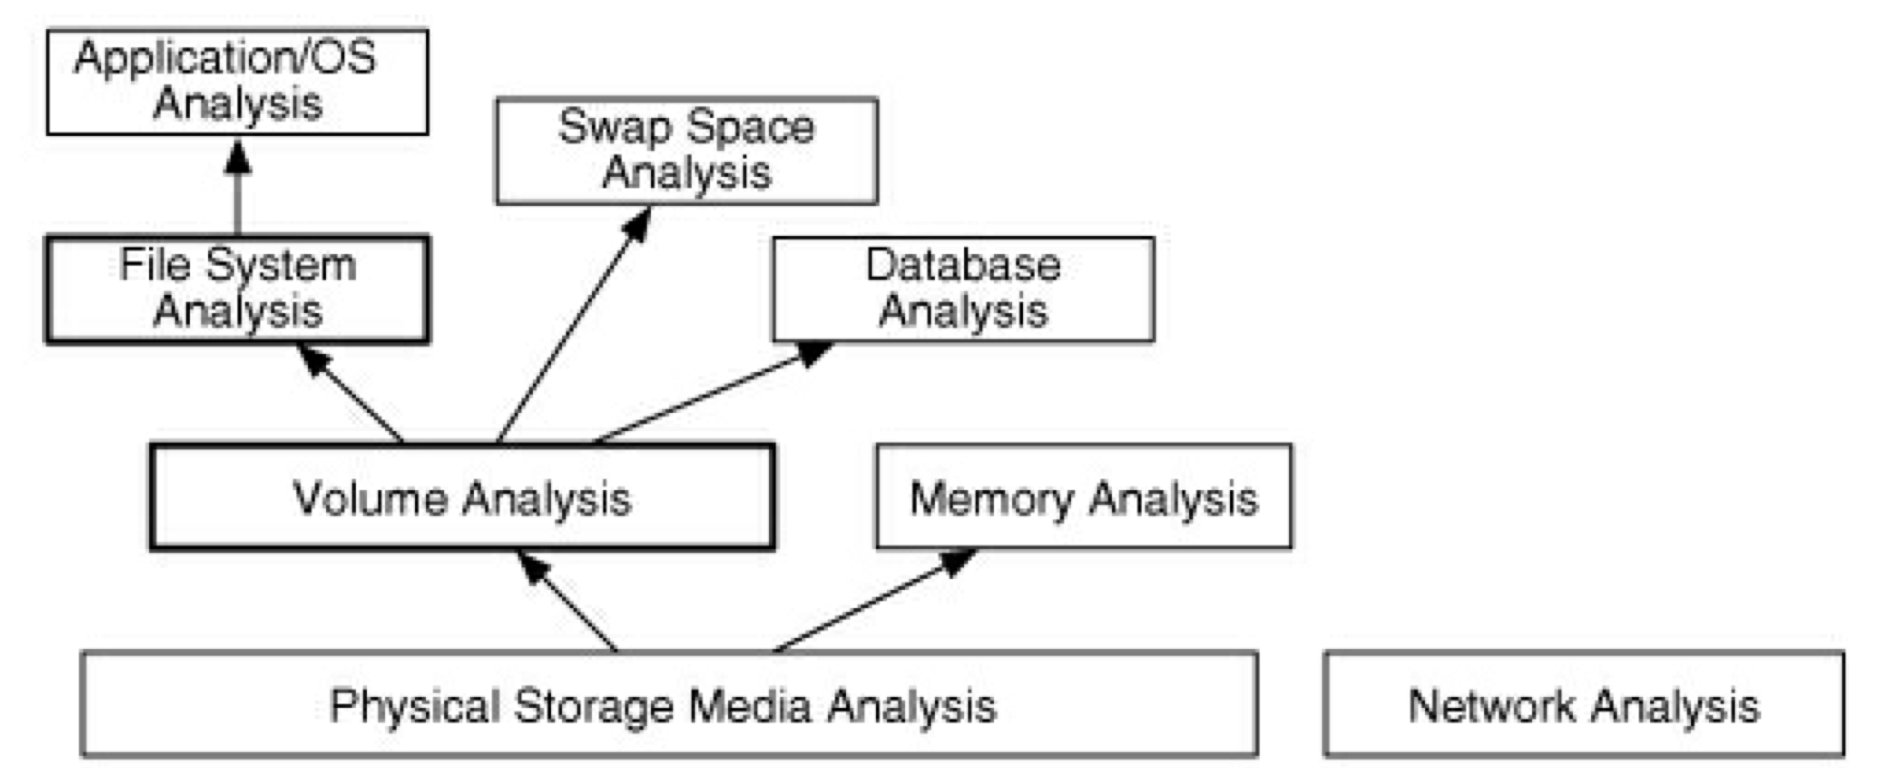
\includegraphics[scale=0.3]{digital-data-analysis-layers-BrianCarrier}
		\caption{Layers of Analysis}
	\end{figure}
\end{frame}

\begin{frame}% Title Page
	\section{Forensic Process}
	\begin{center}
		\Huge\textbf{Forensic Process}
	\end{center}
\end{frame}

\begin{frame}
	\frametitle{Forensic Process}
	Digital forensics results can be used in a court of law therefore accuracy, integrity and an unbiased approach towards evidence is required.\\
	As a result similar approaches to evidence handling and procedure from traditional forms of forensics are utilised.   
	\begin{block}{Scientific Method}
		Defining a hypothesis based on evidence then proceeding search for evidence which disproves our hypothesis.
	\end{block}
	\begin{block}{Digital Forensic Investigation}
	``A digital forensic investigation is a process that uses science
     and technology to analyse digital objects and that develops and
     tests theories, which can be entered into a court of law, to
     answer questions about events that occurred. In other words, a
     digital forensic investigation is a more restricted form of
     digital investigation.'' - Brian Carrier
	\end{block}
\end{frame}

\begin{frame}[fragile]
	\frametitle{Digital Crime Scene Investigation Process Overview}
	\subsection*{Digital Crime Scene Investigation Process Overview}
	There are three major areas in digital crime scene investigations:
	\begin{itemize}
		\item System Preservation
		\item Evidence Searching
		\item Event Reconstruction
	\end{itemize}
	\begin{figure}
		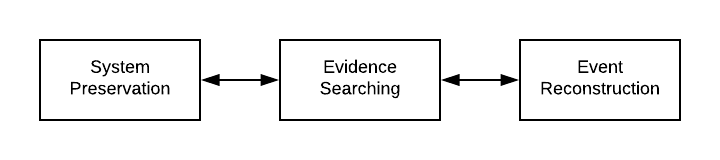
\includegraphics[scale=1]{df-guidelines}
		\caption{Diagram of Digital Forensics Investigation Phases}
		\label{fig:df-guidelines}
	\end{figure}
\end{frame}

\begin{frame}
	\frametitle{PICL Guidelines}
	\subsection*{PICL Guidelines}
	While each forensic investigator/team may have their own procedures and work flow the PICL guidelines below provide a good staring structure:
	\begin{itemize}
		\item Preservation:	 Preservation of the system being investigated.
		\item Isolation:	 Keeping analysis environment is separate from both the suspect data and the outside world.
		\item Correlation:	 Correlate data with other independent sources. Reduces risk of forged data.
		\item Logging:	 Log/document your actions. This helps identify what searches you have not yet conducted and what your results were.
	\end{itemize}
\end{frame}

\begin{frame}
	\frametitle{Analysis Types}
	\subsection*{Analysis Types}
	\begin{block}{Live Analysis:}
		``A live analysis occurs when you use the operating system or other resources of the system being investigated to find evidence.'' - Brian Carrier
	\end{block}

	\begin{block}{Dead Analysis:}
		``A dead analysis occurs when you are running trusted applications in a trusted operating system to find evidence.'' - Brian Carrier
	\end{block}
\end{frame}

\begin{frame} %Title Page
	\section{Forensic Imaging}
	\begin{center}
		\Huge\textbf{Forensic Imaging}
	\end{center}
\end{frame}

\begin{frame}
	\frametitle{Evidence Acquisition/Imaging}
	\begin{itemize}
		\item In order to perform analysis on digital artefacts a forensic duplicate of the media must be created.
		\item Forensic Duplicates are \emph{bit-for-bit} copies of the original disk and can encompass the full disk or a single partition. 
		\item This process is known as imaging or acquisition.
		\item Contents of a disk are always changing therefore \emph{Write Blockers} are used to preserve the disk state.
		\item Hash functions such as SHA-256, SHA-1, MD5 are used to verify the image against the original artefact.
	\end{itemize}
\end{frame}

\begin{frame}
	\frametitle{Write Blockers}
	\subsection*{Write Blockers}
	\begin{block}{Write Blockers}
			Are hardware or software devices that allow gathering of information without damaging the disk contents by blocking write commands but allowing read commands.
	\end{block}
	\begin{itemize}
		\item Write Blockers are customisable:
			\begin{itemize}
				\item Blocking of all or specific commands.
				\item Can control the read and write speed.
			\end{itemize}
		\item Write Blockers come in two forms:
			\begin{itemize}
				\item \emph{Native}: Same interface for input and output e.g. IDE-to-IDE
				\item \emph{Tailgate}: uses different interfaces for input and output e.g. firewire/USB-to-SATA
			\end{itemize}
		\end{itemize}
\end{frame}

\begin{frame}
	\frametitle{Imaging Challenges with Solid State Drives (SSD)}
	\subsection*{Imaging Challenges}
	While an SSD can be imaged with the same tools as a traditional hard disk drive (HDD), there are technology specific issues that cause problems for forensic investigators.
	\begin{itemize}
		\item \emph{Program-Erase cycles}
			\begin{itemize}
				\item Sequence of events that result in data being written to a solid state flash memory cell, then erased and rewritten (e.g flash memory USB sticks). 
				\item These P/E cycles result in a small amount of physical damage to the medium, which can result in bad sectors.
			\end{itemize}
		\item \emph{Wear Levelling}
			\begin{itemize}
				\item prolongs the life of solid state/flash memory
				\item Distributes rewrites evenly across the medium, so no single block dies prematurely.
			\end{itemize}
		\item These two technologies due to the evolution of memory results in unallocated space being overwritten earlier than it would on a HDD. This could overwrite valuable hidden information by accident
	\end{itemize}
\end{frame}

\begin{frame}
	\frametitle{Image Types}
	\subsection*{Image Types}
	\begin{itemize}
		\item Raw Format (\texttt{.dd} \texttt{.raw} \texttt{.img})
		\begin{itemize}
			\item only contain data from the original artifact
			\item meta data is no included however can be generated into a separate file by tools.
			\item Tools: \texttt{dd}, \texttt{dcfldd}, \texttt{dd\_rescue}, \texttt{rdd}, \texttt{df3dd}, \texttt{guymager}
		\end{itemize}
		\item EnCase Evidence Format (Expert Witness \texttt{.E01})
		\begin{itemize}
			\item Expert Witness images use headers and footers to hold metadata about the image.
			\item metatdata can include: drive type, source disk OS, timestamps, hashes, CRCs over blocks.
		\end{itemize}
	\end{itemize}
\end{frame}

\begin{frame}% Title Page
	\section{File Systems}
	\begin{center}
		\Huge\textbf{File Systems}
	\end{center}
\end{frame}

\begin{frame}[allowframebreaks]
	\frametitle{What are File Systems?}
	\begin{block}{File System:}
		File systems manage how data is stored and retrieved in a computer system. They consist of structural and user data which can be organised and understood by users and computers.
	\end{block}
	
	\begin{itemize}
		\item File system architectures (FAT32, Ext3 etc.) provide different methods of tracking data on physical media each has their own data structures, look up tables and allocation methods. \\
		
		\item Modern operating systems contain support for many different file systems providing an interface with physical storage. 
	\end{itemize}
	
	\newpage
	File systems are made up of 2/3 layers:
	\begin{enumerate}
		\item\textbf{Logical Layer}: Provides a user application level API for commands such as read, write and chmod etc.
		\item\textbf{Virtual Layer}\textit{optional}: Allows access to multiple physical file systems e.g. block based: FAT32, NTFS or network based: NFS
		\item\textbf{Physical Layer}: Interacts with hardware, performing block and memory management and interacting with device drivers etc.
	\end{enumerate}
	
	\begin{figure}[h]
		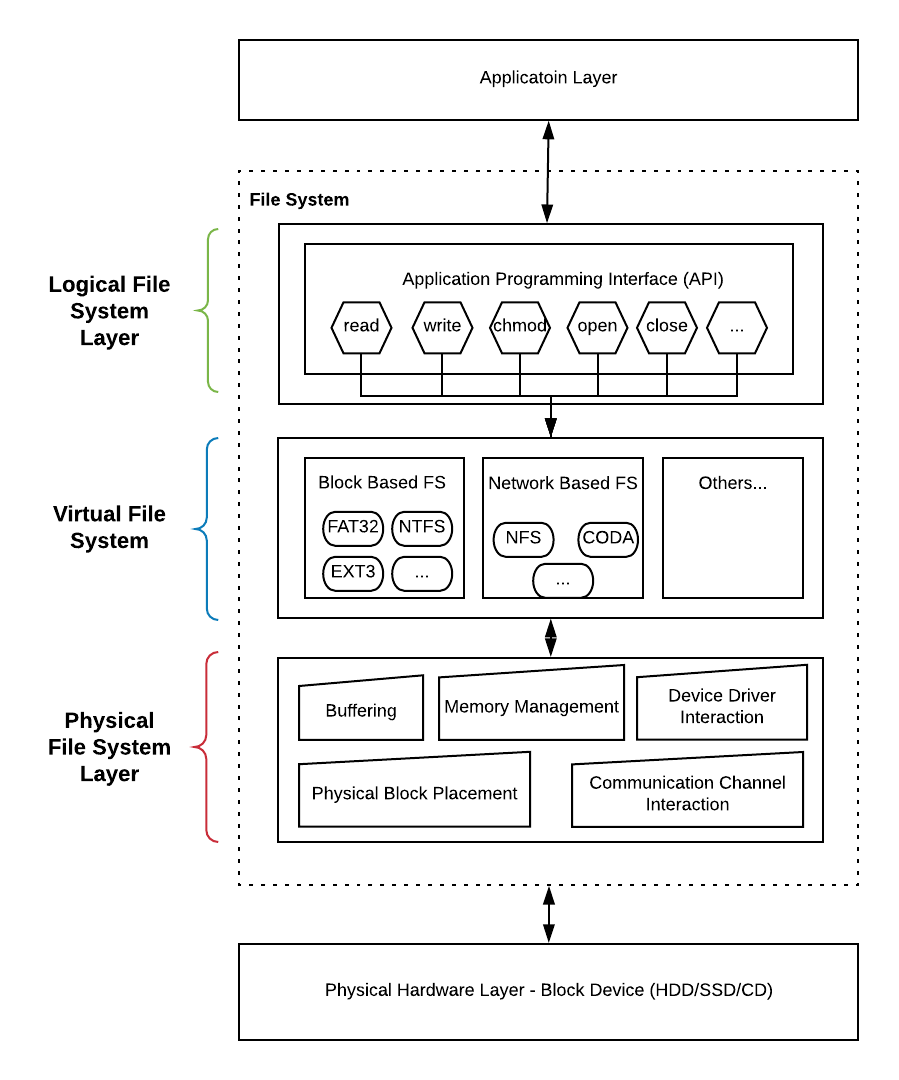
\includegraphics[scale=0.5]{abstract-fs-diagram}
		\caption{Abstract Diagram of a File System on a Computer}
		\label{fig:abstract-fs-diagram}	
	\end{figure}

	
	%TODO enter diagram of how file system interacts with os and hardware
	%TODO add info on volumes and different addressing types in file systems
		
%	\section{Hard Disk Technology}
%		\subsection{Memory Types} %HDD SSD NAND-Flash
%		\subsection{Forensics Memory Challenges}
\end{frame}

\begin{frame}
	\frametitle{File Systems Terminology}
	\subsection*{File System Terminology}
	\begin{itemize}
		\item{\textbf{Sector}}:\\ Smallest addressable section of memory, which holds static amount of data (512/2048/4096-bytes)
		%\item\textbf{Volume}:\\ 
		\item\textbf{INode}:\\ Data structure in a file system that contains meta data (a.k.a Meta Data Pointers/Structures)
		\item\textbf{Data Unit}:\\ Standard sized container for storing \textit{content} data,which consists of multiple \textbf{sectors}. Different file systems have different names for these data units e.g. (Cluster or Block). 
	\end{itemize}
\end{frame}

\begin{frame}
	\frametitle{File System Aspects/Categories}
	\subsection*{File System Categories}
	Each file system contains elements from the following categories:
	\begin{itemize}
		\item \textbf{File System}: \\ Contains file system structure overview and where to find other structures and important data.
		\item \textbf{Content}: \\ Contains data relating to actual file contents, these are usual organised into containers called data units (block/cluster).
		\item \textbf{Meta data}: \\ Data that describes files such as access times, file size, users.
		\item \textbf{File Name}: \\ Contains the data that assigns a name to a file, is used by users instead of a meta data address.
		\item \textbf{Application}: \\ Special features/additional functionality such as quota data or journalling.	
	\end{itemize}	    
\end{frame}

\begin{frame}
	\frametitle{File System Categories Interaction}
	\begin{figure}[h]
		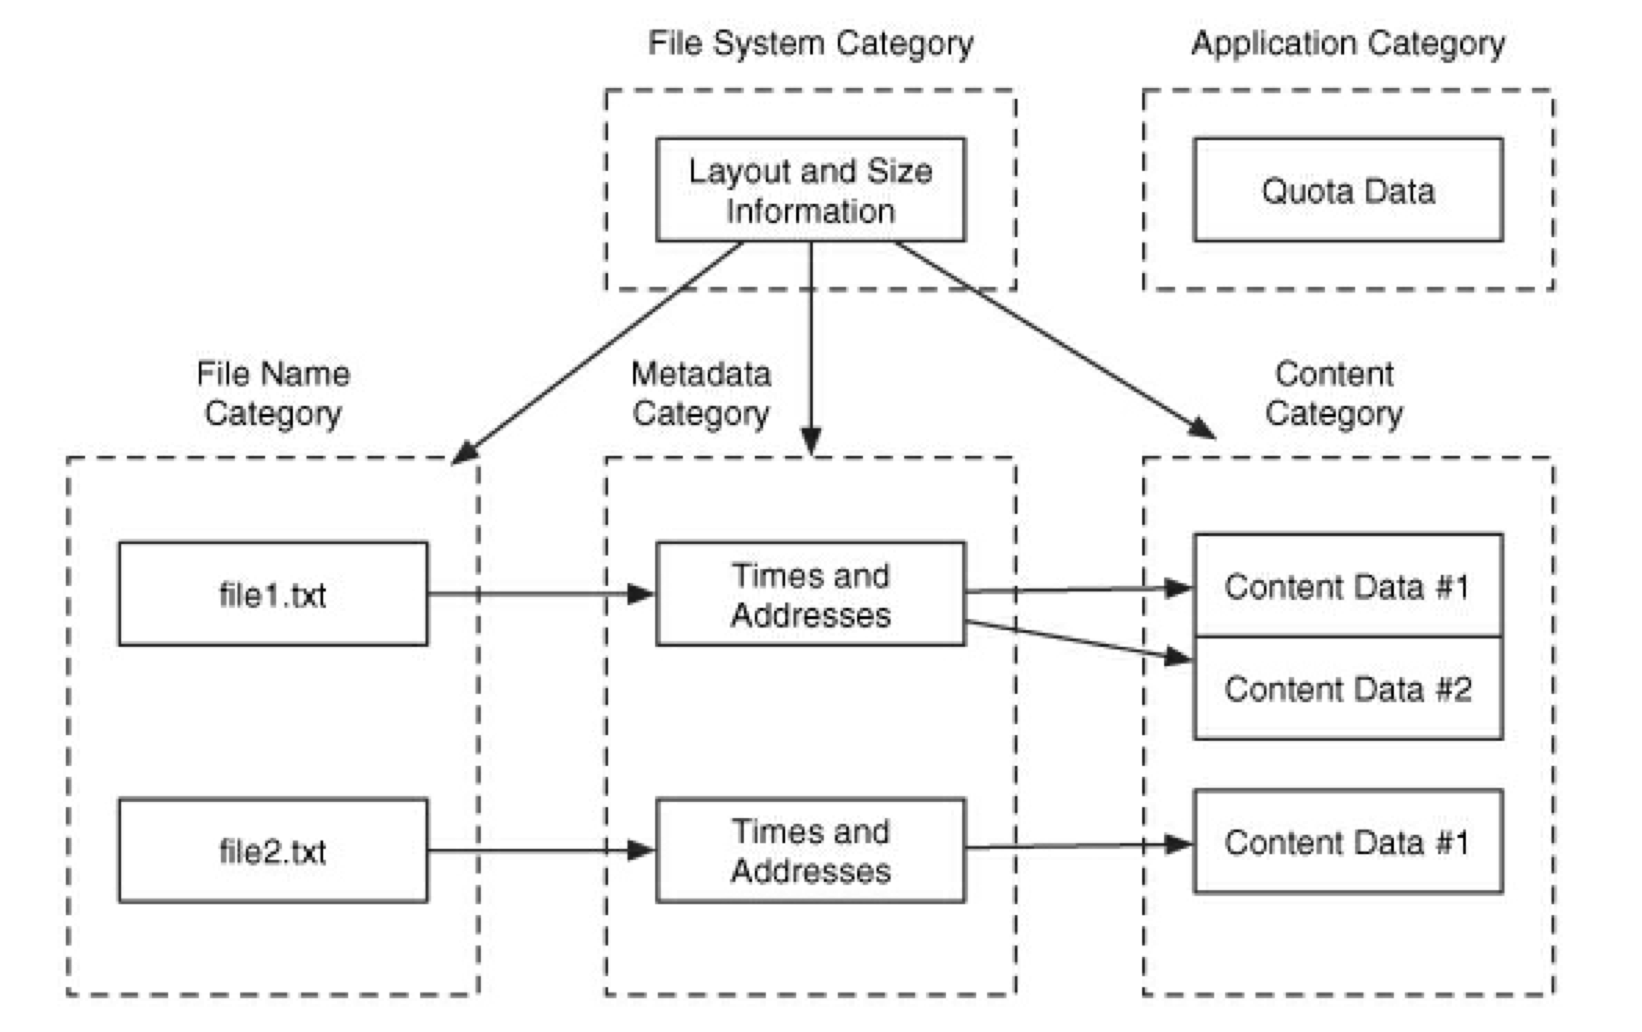
\includegraphics[scale=0.40]{fs-category-interaction-briancarrier}
		\caption{File System Categories Interaction}
		\label{fig:fs-category-interaction}
	\end{figure}
\end{frame}

\begin{frame}
	\frametitle{File System Categories By Example}
	\begin{figure}[h]
		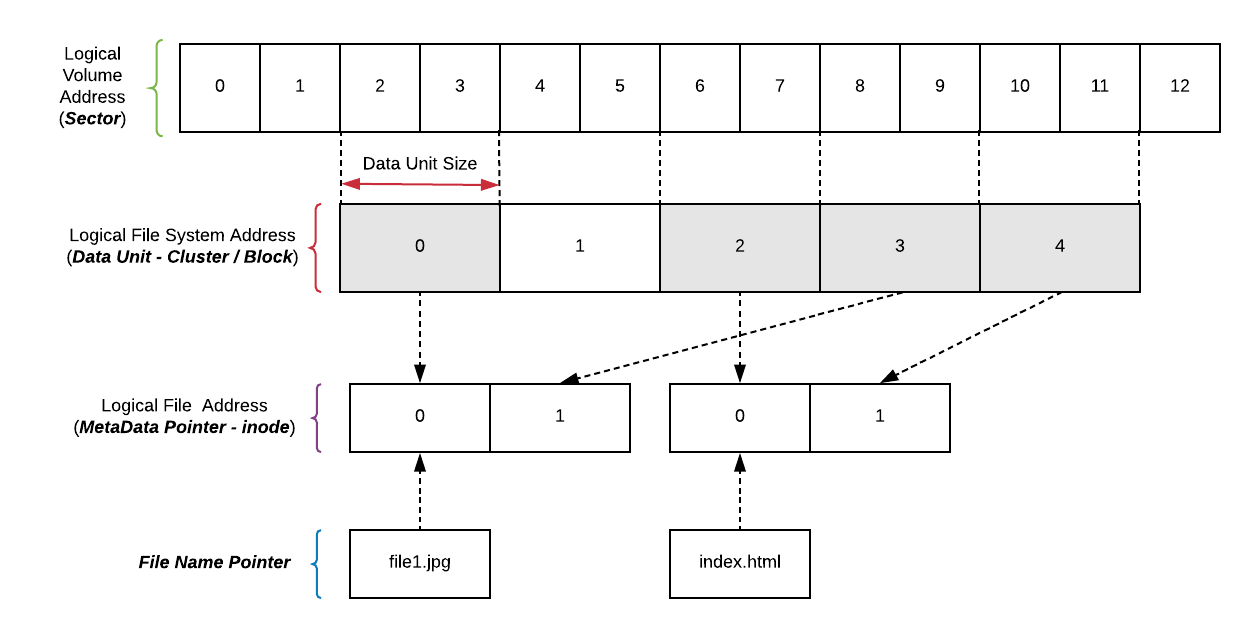
\includegraphics[scale=0.65]{file-system-example}
		\caption{File System Example}
		\label{fig:fs-example}
	\end{figure}
\end{frame}

\begin{frame}
	\frametitle{File System Architectures}
	\section*{File System Architectures}
	There are numerous file system architectures available, some are operating system specific others are designed to be more universal. \\
	
	Examples include:
	\begin{itemize}
		\item FAT - File Allocation Table (FAT8/16/32) - Commonly found on Removable Media 
		\item NTFS - New Technology File System - Default For Windows
		\item Ext - Extended File System (Ext2/3/4) - Default for Linux
	\end{itemize}
	
	
	We will focus on FAT32 in this lecture due to the lab being structured around applying forensic techniques on removable media.
\end{frame}

\begin{frame}
	\frametitle{File Allocation Table 32 - FAT32}
	\section*{File Allocation Table 32 - FAT32}
	There are 
\end{frame}


\begin{frame}% Title Page
	\section{File System Analysis}
	\begin{center}
		\Huge\textbf{File System Analysis}
	\end{center}
\end{frame}

\begin{frame}
	\frametitle{File System Analysis Techniques}
	\section*{File System Analysis Techniques}
	There are many different techniques and theory for the aforementioned categories. In the respect of time and scope of the lecture I will only cover the ones that are relevant to the lab materials.
\end{frame}

\begin{frame}% Title Page
	\section{Forensic Tools}
	\begin{center}
		\Huge\textbf{Forensic Tools}\\
		\large\textit{(Used in Accompanying Lab)}
	\end{center}
\end{frame}

\begin{frame}
	\frametitle{Guymager - Forensic Imaging}
	\subsection*{Guymager}
	\begin{block}{Guymager}
		Guymager is a GUI based forensic imaging tool, that allows for the creation of various image types such as Raw (dd) and EnCase (E01).
	\end{block}
	\begin{figure}[h]
		\centering
		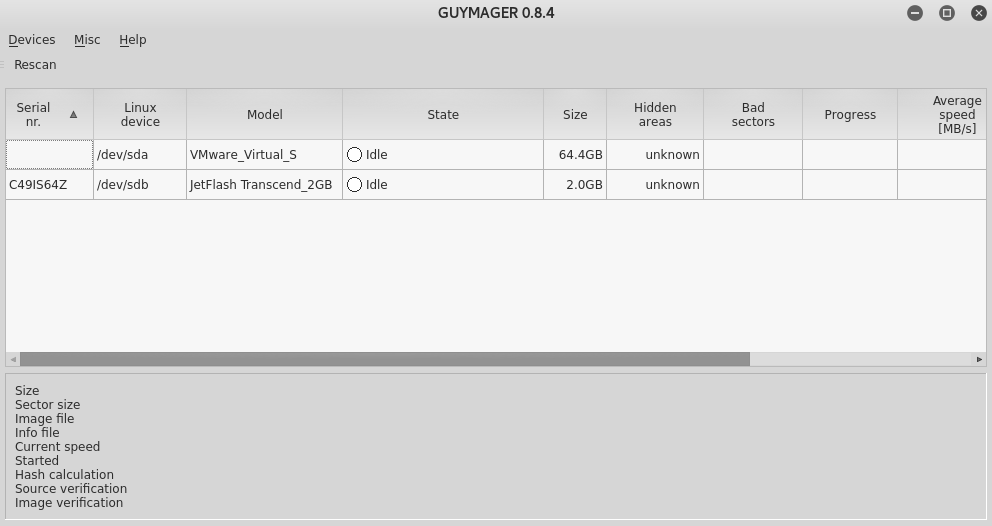
\includegraphics[scale=0.3]{guymager-window}
		\caption{\textit{guymager gui window example}}
		\label{fig:guymager-main-window}
	\end{figure}
\end{frame}

\begin{frame}
	\subsection*{Foremost}
	\frametitle{Foremost - Data Carving}
	\begin{block}{Foremost}
		Foremost is a command line tool that utilises data carving techniques to recover files.
	\end{block}
	\begin{itemize}
		\item \textbf{Data Carving} is a process where files are recovered from a disk image based on common information such as file headers, footers and data structures. 
		\item Performing data carving for large forensic images can be rather tedious if done by hand, tools such as \textbf{Foremost} have been developed to help digital forensic investigators automating this process.
	\end{itemize}
\end{frame}

\begin{frame}
	\subsection*{The Sleuth Kit (TSK)}
	\frametitle{The Sleuth Kit (TSK)\footnote{http://www.sleuthkit.org/}}
	\begin{block}{The Sleuth Kit (TSK)}
	The Sleuth Kit is a series of command line tools that allow users to inspect and analyse disk images and the file systems therein.
	\end{block}
	\begin{itemize}
		\item The tools provided in TSK are divided into the 5 file system categories discussed previously, file system, content (data unit), meta data, file name.
		\item Due to the wide variety of tools within TSK I will discuss those of which we will use in the accompanying lab.
		\item Other features of TSK can befound in the tool overview: \url{http://wiki.sleuthkit.org/index.php?title=TSK_Tool_Overview}
	\end{itemize}
\end{frame}

\begin{frame}
	\frametitle{TSK - File System Layer Tools}
	\subsection*{TSK - File System Layer Tools}
	\begin{itemize}
		\item \textbf{fsstat}: shows file system details and statistics including layout, sizes and labels
	\end{itemize}	
	% either swap to live demo or show annotated print screen explaining information shown
	% give exmaple commands
\end{frame}

\begin{frame}
	\frametitle{TSK - File Name Tools}
	\subsection*{TSK -File Name Tools}
	Allow for processing of file name structures.
	\begin{itemize}
		\item \textbf{ffind}: finds allocated and unallocated file names that point to a given meta data structure
		\item \textbf{fls} lists allocated and deleted file names in a directory
	\end{itemize}		
	% either swap to live demo or show annotated print screen explaining information shown
	% give exmaple commands
\end{frame}

\begin{frame}
	\frametitle{TSK - Meta Data Layer Tools}
	\subsection*{TSK - Meta Data Layer Tools}
	\begin{itemize}
		\item \textbf{icat}: Extracts the data units of a file, which is specified by its meta data address.
		\item \textbf{ifind}: Finds the meta data structure that has a given file name pointing to it or the meta data structure that points to a given data unit.
		\item \textbf{ils}: Lists the meta data structures and their contents in a pipe delimited format.
		\item \textbf{istat}: Displays the statistics and details about a given meta data structure in an easy to read format.
	\end{itemize}
	% either swap to live demo or show annotated print screen explaining information shown
	% give exmaple commands
\end{frame}

\begin{frame}
	\frametitle{TSK - Data Unit Tools}
	\subsection*{TSK - Data Unit Tools}
	These file system tools process the data units where file content is stored.
	\begin{itemize}
		\item \textbf{blkcat}: Extracts the contents of a given data unit.
		\item \textbf{blkls}: Lists the details about data units and can extract the unallocated space of the file system.
		\item \textbf{blkstat}: Displays the statistics about a given data unit in an easy to read format.
		\item \textbf{blkcalc}: Calculates where data in the unallocated space image (from blkls) exists in the original image. This is used when evidence is found in unallocated space.
	\end{itemize}
	% either swap to live demo or show annotated print screen explaining information shown
	% give exmaple commands
\end{frame}

\begin{frame}
	\frametitle{TSK - Volume System Tools}
	\subsection*{TSK - Volume System Tools}
	These tools take a disk (or other media) image as input and analyse its partition structures. 
	\begin{itemize}
		\item \textbf{mmls}: Displays the layout of a disk, including the unallocated spaces.
		\item \textbf{mmstat}: Display details about a volume system (typically only the type).
		\item \textbf{mmcat}: Extracts the contents of a specific volume to STDOUT.
	\end{itemize}
	% either swap to live demo or show annotated print screen explaining information shown
	% give exmaple commands
\end{frame}

%\begin{frame}
%	\section*{Research}
%	\frametitle{Digital Forensic Research}
%\end{frame}

\begin{frame}
	\section{Additional Resources}
	\frametitle{Additional Resources}
	
\end{frame}

\begin{frame}
	\section{Careers}
	\frametitle{Careers}
	
\end{frame}

\end{document} % End Document